\scanpage{11}

% ll. 1–4
\mspage{\textcircled{9}}
Il suffit de prouver que $\alpha_i$ non lié à $\gamma_4$, mais comme il est lié à $\beta_4$, $[\beta_4,\gamma_4]$ serait sinon \deleted{\unsure{point}}\inserted{arête} de deux triangles (de \unsure{sommet|sommets} $\alpha_i$ et $\alpha_4$), cqfd

% upper left
\figure{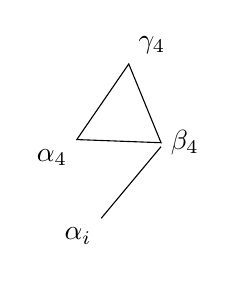
\begin{tikzpicture}[scale=1]
\draw (0,0) node[below left] {$\alpha_4$} -- (.66,.96) node[above right] {$\gamma_4$} -- (1.07,-.04) node[right] {$\beta_4$} -- cycle;
\draw (1.07,-.09) -- (.31,-1) node[below left] {$\alpha_i$};
\end{tikzpicture}}

% l. 5
\uline{Lemme} 9

% ll. 6–8
\diagram{\(\displaystyle\mathrm{III}\left\{\begin{array}{llll}
\alpha_i\ \text{lié à}&\beta_j,\gamma_j,\unsure{\beta'_i},\gamma'_i\ (1\leq i\ne j\leq3)&\text{non à}&\beta'_j,\gamma'_j,\beta_i,\gamma_i\\
\beta_i\ \text{lié à}&\gamma_j,\alpha_j,\unsure{\gamma'_i},\alpha'_i\ (\rule{.7cm}{.35pt})&\rule{.85cm}{.35pt}&\gamma'_j,\alpha'_j,\gamma_i,\alpha_i\\
\gamma_i\ \rule{.8cm}{.35pt}&\alpha_j,\beta_j,\alpha'_i,\beta'_i\ \rule{.7cm}{.35pt})&\rule{.85cm}{.35pt}&\alpha'_j,\beta'_j,\alpha_i,\beta_i.
\end{array}\right.\)}

% ll. 9–11
\diagram{\(\displaystyle\mathrm{III}'\left\{\begin{array}{llll}
\alpha'_i\ \text{lié à}&\beta'_j,\gamma'_j&--&--\\
--&&--&--\\
--&&--&\rule{.38cm}{.35pt}
\end{array}\right.\)}

% ll. 12–14
Il suffit de voir que $\alpha_1$ lié à $\beta_2,\deleted{\beta_3}\beta_3$ \inserted{non à $\beta_1$}. Or

% ll. 13–14 displayed comparison
\[
\begin{aligned}
\alpha_4\ \text{lié à}&\qquad\beta'_1,\beta'_2,\beta'_3,\beta_4\qquad(\text{lemme }8)\\
\alpha_1\ \text{lié à}&\qquad ?\qquad ?\qquad ?\qquad\beta_4
\end{aligned}
\]

% ll. 15–17
\deleted{Donc} l'ens des coïncidences entre $\unsure{w_v(\alpha_1)|\omega_v(\alpha_1)}$ et $w_v(\alpha_4)$ doit être ds la partition $(1,4)(2,3)$, \unsure{ça doit être|ça donc être|se donc être} \deleted{$\beta_4$} $(1,4)$ puisqu'il contient 4, donc

% l. 18
\[
\alpha_1\ \text{lié à}\qquad\beta'_1,\beta_2,\beta_3,\beta_4\qquad\text{cqfd.}
\]

% ll. 19–21
\uline{Conséquence} : $S$ est déterminé par les conditions de départ, à isom. près. \deleted{\illegible{2}} C'est donc un graphe cubique

% bottom centre
\begin{center}cqfd\end{center}

% bottom right
\margin{TSVP}
% archive sheet number: 10
